% Options for packages loaded elsewhere
\PassOptionsToPackage{unicode}{hyperref}
\PassOptionsToPackage{hyphens}{url}
\documentclass[
  ignorenonframetext,
]{beamer}
\newif\ifbibliography
\usepackage{pgfpages}
\setbeamertemplate{caption}[numbered]
\setbeamertemplate{caption label separator}{: }
\setbeamercolor{caption name}{fg=normal text.fg}
\beamertemplatenavigationsymbolsempty
% remove section numbering
\setbeamertemplate{part page}{
  \centering
  \begin{beamercolorbox}[sep=16pt,center]{part title}
    \usebeamerfont{part title}\insertpart\par
  \end{beamercolorbox}
}
\setbeamertemplate{section page}{
  \centering
  \begin{beamercolorbox}[sep=12pt,center]{section title}
    \usebeamerfont{section title}\insertsection\par
  \end{beamercolorbox}
}
\setbeamertemplate{subsection page}{
  \centering
  \begin{beamercolorbox}[sep=8pt,center]{subsection title}
    \usebeamerfont{subsection title}\insertsubsection\par
  \end{beamercolorbox}
}
% Prevent slide breaks in the middle of a paragraph
\widowpenalties 1 10000
\raggedbottom
\AtBeginPart{
  \frame{\partpage}
}
\AtBeginSection{
  \ifbibliography
  \else
    \frame{\sectionpage}
  \fi
}
\AtBeginSubsection{
  \frame{\subsectionpage}
}
\usepackage{iftex}
\ifPDFTeX
  \usepackage[T1]{fontenc}
  \usepackage[utf8]{inputenc}
  \usepackage{textcomp} % provide euro and other symbols
\else % if luatex or xetex
  \usepackage{unicode-math} % this also loads fontspec
  \defaultfontfeatures{Scale=MatchLowercase}
  \defaultfontfeatures[\rmfamily]{Ligatures=TeX,Scale=1}
\fi
\usepackage{lmodern}
\usetheme[]{Madrid}
\usefonttheme[]{professionalfonts}
\ifPDFTeX\else
  % xetex/luatex font selection
\fi
% Use upquote if available, for straight quotes in verbatim environments
\IfFileExists{upquote.sty}{\usepackage{upquote}}{}
\IfFileExists{microtype.sty}{% use microtype if available
  \usepackage[]{microtype}
  \UseMicrotypeSet[protrusion]{basicmath} % disable protrusion for tt fonts
}{}
\makeatletter
\@ifundefined{KOMAClassName}{% if non-KOMA class
  \IfFileExists{parskip.sty}{%
    \usepackage{parskip}
  }{% else
    \setlength{\parindent}{0pt}
    \setlength{\parskip}{6pt plus 2pt minus 1pt}}
}{% if KOMA class
  \KOMAoptions{parskip=half}}
\makeatother
\usepackage{longtable,booktabs,array}
\usepackage{calc} % for calculating minipage widths
\usepackage{caption}
% Make caption package work with longtable
\makeatletter
\def\fnum@table{\tablename~\thetable}
\makeatother
% definitions for citeproc citations
\NewDocumentCommand\citeproctext{}{}
\NewDocumentCommand\citeproc{mm}{%
  \begingroup\def\citeproctext{#2}\cite{#1}\endgroup}
\makeatletter
 % allow citations to break across lines
 \let\@cite@ofmt\@firstofone
 % avoid brackets around text for \cite:
 \def\@biblabel#1{}
 \def\@cite#1#2{{#1\if@tempswa , #2\fi}}
\makeatother
\newlength{\cslhangindent}
\setlength{\cslhangindent}{1.5em}
\newlength{\csllabelwidth}
\setlength{\csllabelwidth}{3em}
\newenvironment{CSLReferences}[2] % #1 hanging-indent, #2 entry-spacing
 {\begin{list}{}{%
  \setlength{\itemindent}{0pt}
  \setlength{\leftmargin}{0pt}
  \setlength{\parsep}{0pt}
  % turn on hanging indent if param 1 is 1
  \ifodd #1
   \setlength{\leftmargin}{\cslhangindent}
   \setlength{\itemindent}{-1\cslhangindent}
  \fi
  % set entry spacing
  \setlength{\itemsep}{#2\baselineskip}}}
 {\end{list}}
\usepackage{calc}
\newcommand{\CSLBlock}[1]{\hfill\break\parbox[t]{\linewidth}{\strut\ignorespaces#1\strut}}
\newcommand{\CSLLeftMargin}[1]{\parbox[t]{\csllabelwidth}{\strut#1\strut}}
\newcommand{\CSLRightInline}[1]{\parbox[t]{\linewidth - \csllabelwidth}{\strut#1\strut}}
\newcommand{\CSLIndent}[1]{\hspace{\cslhangindent}#1}
\setlength{\emergencystretch}{3em} % prevent overfull lines
\providecommand{\tightlist}{%
  \setlength{\itemsep}{0pt}\setlength{\parskip}{0pt}}
\usepackage{xurl}          % better URL/DOI wrapping
\usepackage{microtype}     % nicer spacing
\setbeamertemplate{bibliography item}[text]  % no bullets on refs
\usepackage{bookmark}
\IfFileExists{xurl.sty}{\usepackage{xurl}}{} % add URL line breaks if available
\urlstyle{same}
\hypersetup{
  pdftitle={An adaptive test based on Kendall's tau for independence in high dimensions},
  pdfauthor={Sam Olson},
  hidelinks,
  pdfcreator={LaTeX via pandoc}}

\title{An adaptive test based on Kendall's tau for independence in high
dimensions}
\author{Sam Olson}
\date{}

\begin{document}
\frame{\titlepage}

\begin{frame}{Synopsis of Paper}
\phantomsection\label{synopsis-of-paper}
\begin{itemize}
\tightlist
\item
  Testing the mutual independence for high-dimensional data.
\item
  Known that \(L_2\)-type statistics have lower power under sparse
  alternatives in high dimensions
\item
  Also known that \(L_\infty\)-type statistics have lower power under
  dense alternatives in high dimensions
\item
  Goal: Develop an adaptive test based on Kendall's \(\tau\) to work
  well in both situations
\item
  In developing an adaptive test, determine necessary assumptions and
  the asymptotic null distribution of the proposed statistic
\item
  Assess how well the test does compared to other testing methods
\item
  Results indicate the adaptive test performs well in either dense or
  sparse cases
\end{itemize}
\end{frame}

\begin{frame}{What is Kendall's \(\tau\)}
\phantomsection\label{what-is-kendalls-tau}
\[
\tau = \frac{(\text{Count of concordant pairs}) - (\text{Count of discordant pairs})}{(\text{Number of pairs})}
\]

\begin{itemize}
\tightlist
\item
  Note: Any pair of observations \((x_i, y_i)\) and \((x_j, y_j)\),
  where i \textless{} j, are said to be \emph{concordant} if the sort
  order of \((x_i, x_j)\) and \((y_i, y_j)\) agrees
\item
  That is, if either both \(x_i > x_j\) and \(y_i > y_j\) holds or both
  \(x_i < x_j\) and \(y_i < y_j\); otherwise they are said to be
  \emph{discordant}.
\item
  There are other types of Kendall's \(\tau\), e.g., \(\tau_a\),
  \(\tau_b\), and \(\tau_c\)
\end{itemize}
\end{frame}

\begin{frame}{How Does This Fit Into a Broader Narrative?}
\phantomsection\label{how-does-this-fit-into-a-broader-narrative}
\begin{itemize}
\tightlist
\item
  \textbf{1897} --- (Fechner 1897) introduces the \emph{method of signs}
  for succession-dependence.
\item
  \textbf{1938} --- (Kendall 1938) develops the \(\tau\) rank
  correlation coefficient.
\item
  \textbf{1958} --- (Kruskal 1958) broadens Kendall's ideas into a
  general nonparametric testing framework.
\item
  \textbf{1958--1990s} --- Others apply rank-based methods to time
  series (El-Shaarawi and Niculescu 1992; Hamed 2011).
\item
  \textbf{2024} --- (Shi et al. 2024), the focus of this presentation,
  develop adaptive high-dimensional independence tests using Kendall's
  \(\tau\).
\item
  \textbf{2025} --- (Han, Ma, and Xie 2025) extend to a broader class of
  sum-of-powers tests.
\end{itemize}
\end{frame}

\begin{frame}{In Detail: Shi et al.~(2024): Problem Statement}
\phantomsection\label{in-detail-shi-et-al.-2024-problem-statement}
\[
H_0: X_1, \dots, X_d \text{ are mutually independent}
\]

Testing full independence in \textbf{high dimensions} (\(d \gg n\)),
where both \emph{dense} and \emph{sparse} alternatives may occur.
\end{frame}

\begin{frame}{Why Kendall's \(\tau\)?}
\phantomsection\label{why-kendalls-tau}
\begin{itemize}
\tightlist
\item
  \textbf{Rank-based}, \textbf{distribution-free}, and robust to
  \textbf{heavy tails}.\\
\item
  Works even when moments (e.g., variances) are infinite.\\
\item
  Avoids dependence on the data-generation process---no parametric
  assumptions.\\
\item
  Each \(\tau_{k\ell}\) measures pairwise monotonic dependence between
  \(X_k, X_\ell\).
\end{itemize}
\end{frame}

\begin{frame}{How Is This Non-Parametric?}
\phantomsection\label{how-is-this-non-parametric}
\begin{itemize}
\tightlist
\item
  We make no distributional assumptions of the variables (covariates or
  otherwise) we wish to test for independence.
\item
  Doesn't mean the statistic (Kendall \(\tau\)) is distribution-free
  though! Just the inputs going into it!
\end{itemize}
\end{frame}

\begin{frame}{Dense vs.~Sparse Settings}
\phantomsection\label{dense-vs.-sparse-settings}
\begin{longtable}[]{@{}lll@{}}
\toprule\noalign{}
Setting & Dependence Structure & Suitable Statistic \\
\midrule\noalign{}
\endhead
\textbf{Dense} & Many weak correlations & \(L_2\)-type (sum-type) \\
\textbf{Sparse} & Few strong correlations & \(L_\infty\)-type
(max-type) \\
\bottomrule\noalign{}
\end{longtable}
\end{frame}

\begin{frame}[allowframebreaks]{Method (Overview)}
\phantomsection\label{method-overview}
\begin{enumerate}
\tightlist
\item
  Compute pairwise Kendall's taus \(\tau_{k\ell}\).\\
\item
  Construct two base statistics:
\end{enumerate}

\begin{itemize}
\tightlist
\item
  \(S_\tau\) (\(L_2\)-type):
\end{itemize}

\[
S_\tau = \omega_2^{-1/2}\!\left(\sum_{k>\ell}\tau_{k\ell}^2 - \tfrac{d(d-1)}{2}\omega_1\right)
\Rightarrow S_\tau \overset{d}{\to} N(0,1)
\]

\begin{itemize}
\tightlist
\item
  \(M_\tau\) (\(L_\infty\)-type):
\end{itemize}

\[
M_\tau = \omega_1^{-1}\max_{k<\ell}\tau_{k\ell}^2 - 4\ln d + \ln\ln d
\Rightarrow M_\tau \overset{d}{\to} \text{Gumbel}
\]

Where \(\omega_1, \omega_2\) are constants reflecting the variance
structure of pairwise Kendall's \(\tau\)'s under independence.

\begin{enumerate}
\setcounter{enumi}{2}
\tightlist
\item
  Combine the two via the \emph{minimum p-value approach} (an ``adaptive
  test''):
\end{enumerate}

\[
C_\tau = \min\{1 - \Phi(S_\tau),\, 1 - F_{\mathrm{Gumbel}}(M_\tau)\}
\]

What is an Adaptive Test?

\begin{itemize}
\tightlist
\item
  A single procedure that \textbf{automatically adapts} to the
  dependence pattern.\\
\item
  If data are \textbf{dense}, \(S_\tau\) dominates; if \textbf{sparse},
  \(M_\tau\) dominates.\\
\item
  \(C_\tau\) effectively selects the stronger signal through
  \(p\text{-value} = \min(p_{S_\tau}, p_{M_\tau})\).
\end{itemize}
\end{frame}

\begin{frame}{Theoretical Results I}
\phantomsection\label{theoretical-results-i}
With all the following base assumptions:

\begin{itemize}
\tightlist
\item
  Finite 8th moment (for asymptotic normality of \(\tau\) to hold)
\item
  Dependence boundedness conditions (\(\alpha\)-mixing type)
\item
  \(\frac{d}{n} \rightarrow \infty\) allowed
\end{itemize}

Then, \textbf{Under} \(H_0\):

\begin{itemize}
\tightlist
\item
  \(S_\tau\) and \(M_\tau\) are \textbf{asymptotically independent} ---
  key innovation.
\item
  Therefore,
\end{itemize}

\[
(S_\tau, M_\tau) \xrightarrow{d} (Z_1, Z_2)
\quad \text{with } Z_1\sim N(0,1),\; Z_2\sim \text{Gumbel}.
\]
\end{frame}

\begin{frame}{Theoretical Results II}
\phantomsection\label{theoretical-results-ii}
\begin{itemize}
\tightlist
\item
  Consequently,
\end{itemize}

\[
C_\tau = \min\{1 - \Phi(Z_1),\, 1 - F(Z_2)\} \xrightarrow{d} W=\min(U_1,U_2),
\]

where \(U_1,U_2\sim \text{Uniform}(0,1)\).

\[
\Rightarrow H(t) = 2t - t^2,\quad t\in[0,1].
\]

\textbf{Decision rule:}\\
Reject \(H_0\) if \(C_\tau < 1 - \sqrt{1 - \alpha}\).
\end{frame}

\begin{frame}{Practical Implementation}
\phantomsection\label{practical-implementation}
\begin{itemize}
\tightlist
\item
  Two variants:

  \begin{itemize}
  \tightlist
  \item
    \(TC_\tau\): uses theoretical (asymptotic) critical values.\\
  \item
    \(MC_\tau\): uses Monte Carlo--simulated critical values
    (finite-sample accurate).\\
  \end{itemize}
\item
  Distribution-free; efficient table lookup possible for \((n,d)\).
\end{itemize}
\end{frame}

\begin{frame}{Key Properties of the Adaptive Test}
\phantomsection\label{key-properties-of-the-adaptive-test}
\begin{itemize}
\tightlist
\item
  Joint Asymptotic independence of \(S_{\tau}, M_{\tau}\) allows for an
  adaptive combination (hence the valid statistical test of
  independence)
\item
  \textbf{Distribution-free:} No parametric or moment assumptions.\\
\item
  \textbf{Robust:} Handles heavy-tailed or non-Gaussian data.\\
\item
  \textbf{Adaptive:} Unified test for both dense and sparse
  dependence.\\
\item
  \textbf{Asymptotic theory:}

  \begin{itemize}
  \tightlist
  \item
    \(S_\tau \to N(0,1)\)\\
  \item
    \(M_\tau \to \text{Gumbel}\)\\
  \item
    \(S_\tau, M_\tau\) independent\\
  \item
    \(C_\tau \to W\) with \(H(t) = 2t - t^2\)
  \end{itemize}
\end{itemize}
\end{frame}

\begin{frame}{Results I}
\phantomsection\label{results-i}
Under various settings, we compare the following methods:

\begin{itemize}
\item
  \(S_r\): Pearson--correlation \(L_2\)-type test; best for \emph{dense
  dependence}.
\item
  \(TS_{\tau}\): Kendall's tau \(L_2\)-type test using \emph{asymptotic}
  critical values.
\item
  \(MS_{\tau}\): Same as \(TS_{\tau}\) but with \emph{Monte Carlo}
  critical values.
\item
  \(M_r\): Pearson--correlation \(L_{\infty}\)-type test; best for
  \emph{sparse dependence}.
\item
  \(TM_{\tau}\): Kendall's tau \(L_{\infty}\)-type test using
  \emph{asymptotic} Gumbel limits.
\item
  \(MM_{\tau}\): Same as \(TM_{\tau}\) but with \emph{Monte Carlo}
  critical values.
\item
  \(TC_{\tau}\): \emph{Adaptive} Kendall's tau test combining
  \(S_{\tau}\) and \(M_{\tau}\) (asymptotic).
\item
  \(MC_{\tau}\): \emph{Adaptive} Kendall's tau test combining
  \(S_{\tau}\) and \(M_{\tau}\) (Monte Carlo).
\item
  \(PE_r\): \emph{Power-enhanced} Pearson test improving \(S_r\) under
  sparse cases.
\item
  \(U_{\min}\): \emph{Adaptive U-statistic} test combining multiple
  orders via minimum p-value.
\end{itemize}
\end{frame}

\begin{frame}{Results II}
\phantomsection\label{results-ii}
There are a number of tables for the various conditions the author's
tested the statistical tests. The main focus is on the \emph{Size} and
\emph{Power} (mainly the latter) of the statistical tests.

Overall:

\begin{itemize}
\tightlist
\item
  While one particular non-adaptive test may do best under a particular
  setting (dense/sparse),
\item
  Both implementations of the adaptive test proposed does as good (is
  roughly as powerful) as the ``best'' method, but for \textbf{both}
  settings
\item
  Highlighted portions of the tables that follow are the adaptive tests
\end{itemize}
\end{frame}

\begin{frame}{Results III}
\phantomsection\label{results-iii}
\begin{figure}

{\centering 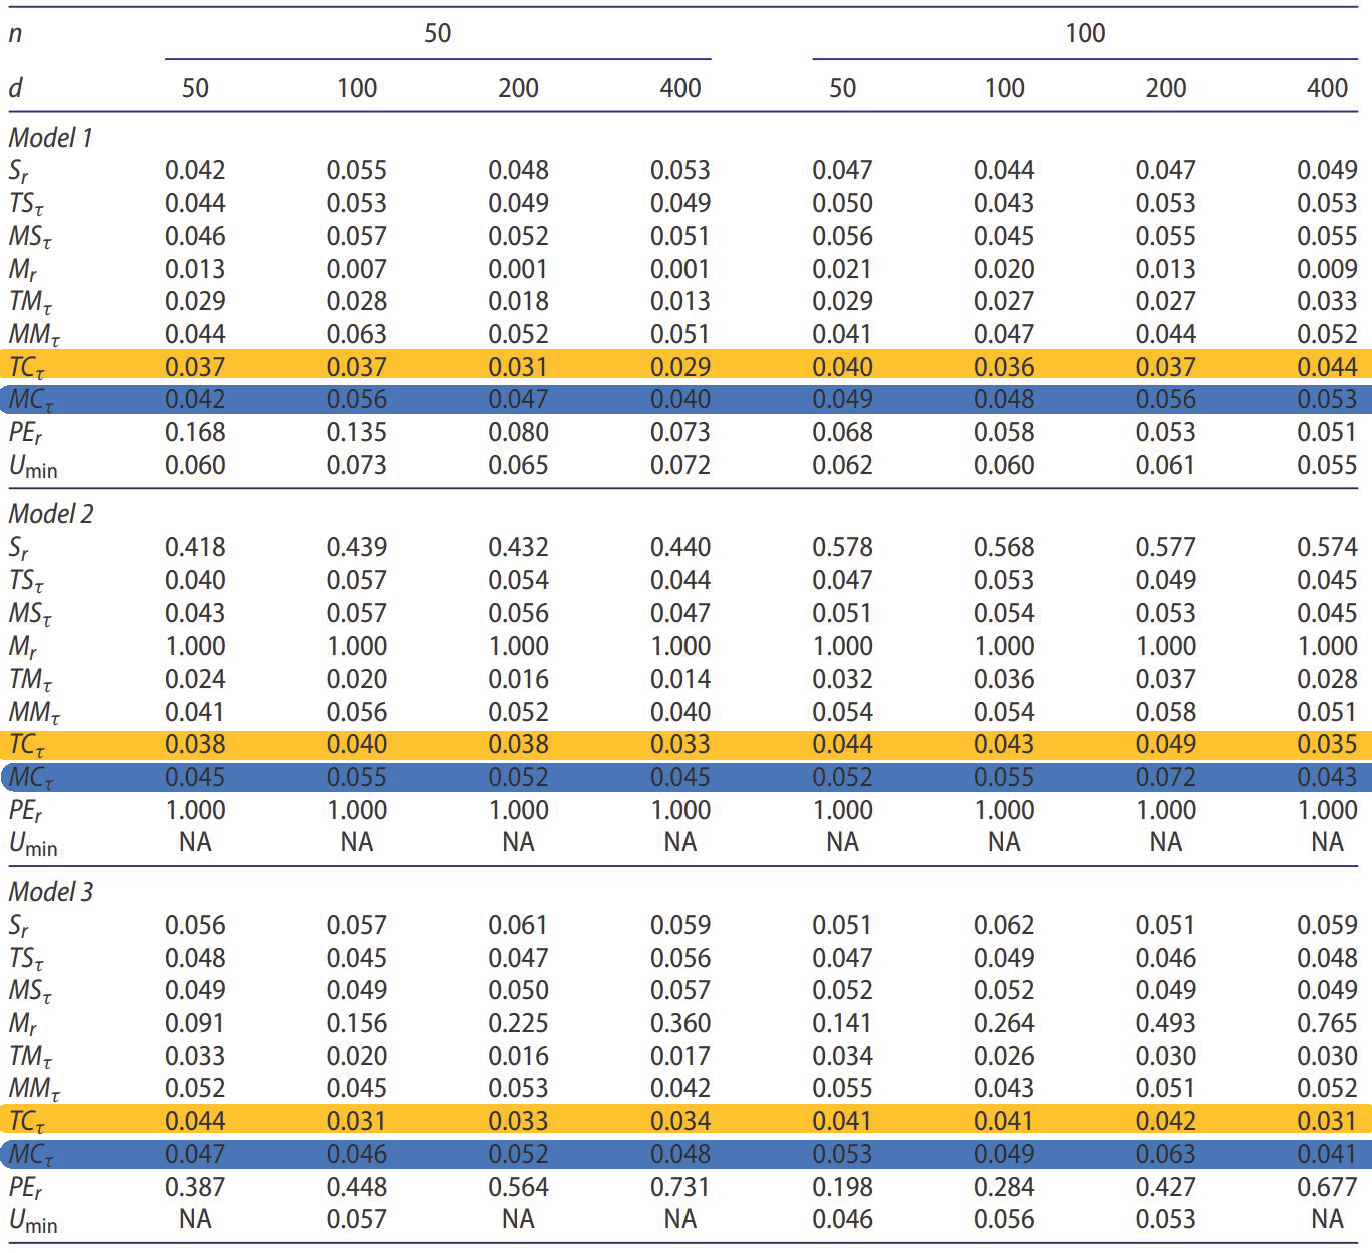
\includegraphics[width=0.8\linewidth,height=0.77\textheight]{Figures/Table1H} 

}

\caption{Empirical sizes of tests}\label{fig:Table 1}
\end{figure}
\end{frame}

\begin{frame}{Results IV}
\phantomsection\label{results-iv}
\begin{figure}

{\centering 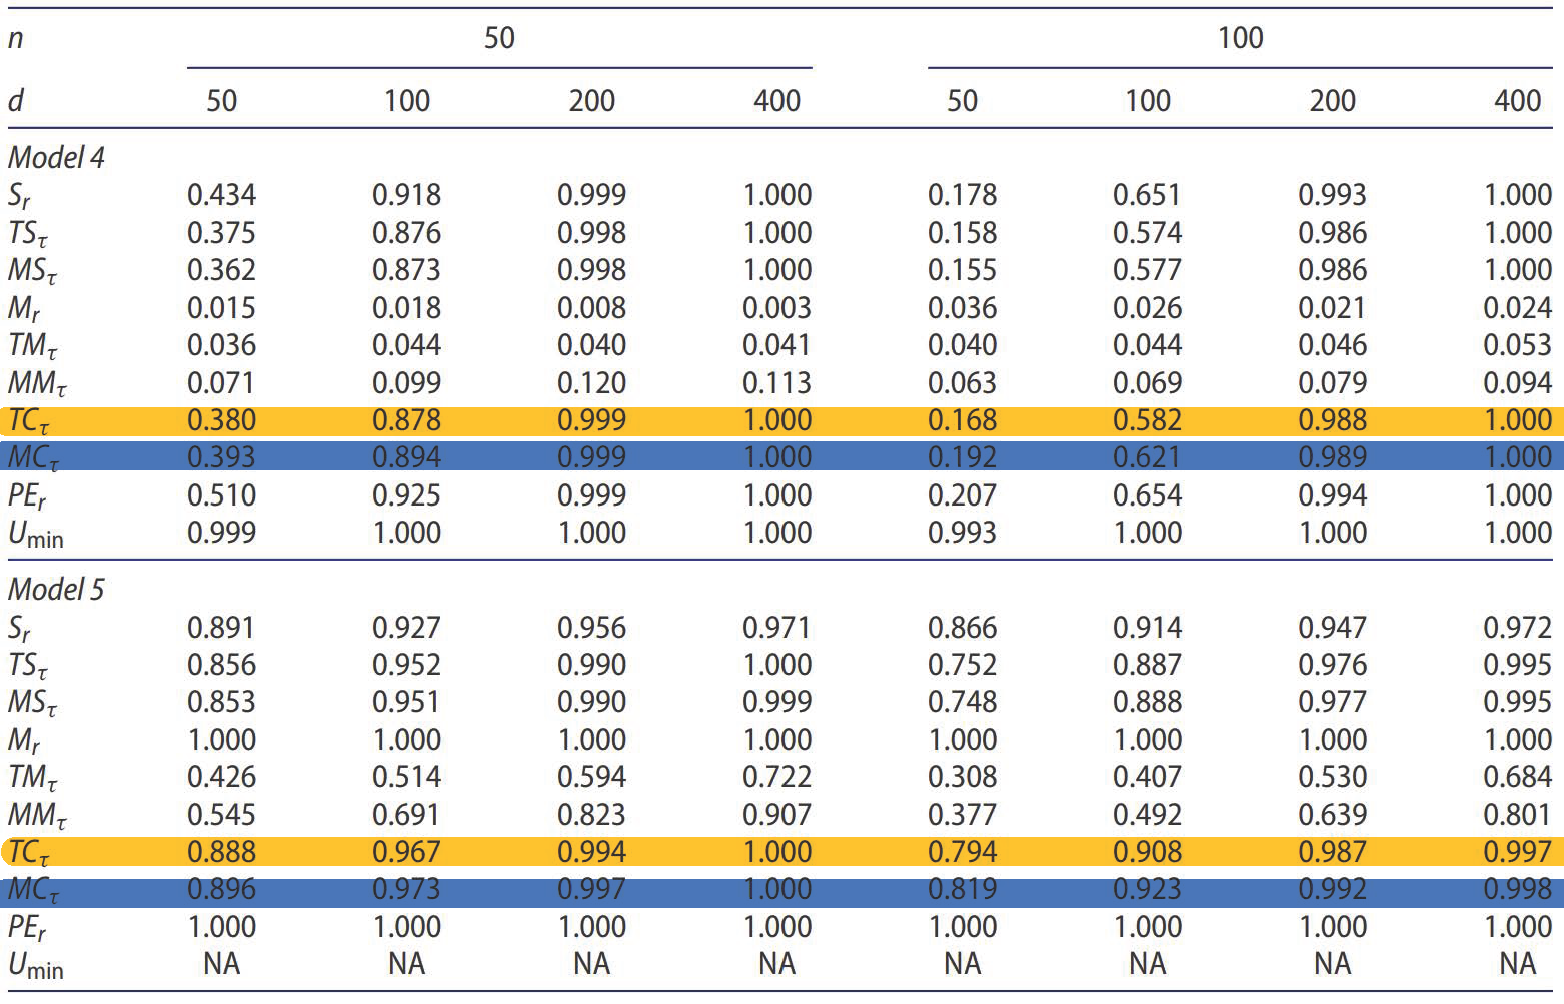
\includegraphics[width=0.8\linewidth]{Figures/Table2H} 

}

\caption{Empirical powers of tests in dense cases.}\label{fig:Table 2}
\end{figure}
\end{frame}

\begin{frame}{Results V}
\phantomsection\label{results-v}
\begin{figure}

{\centering 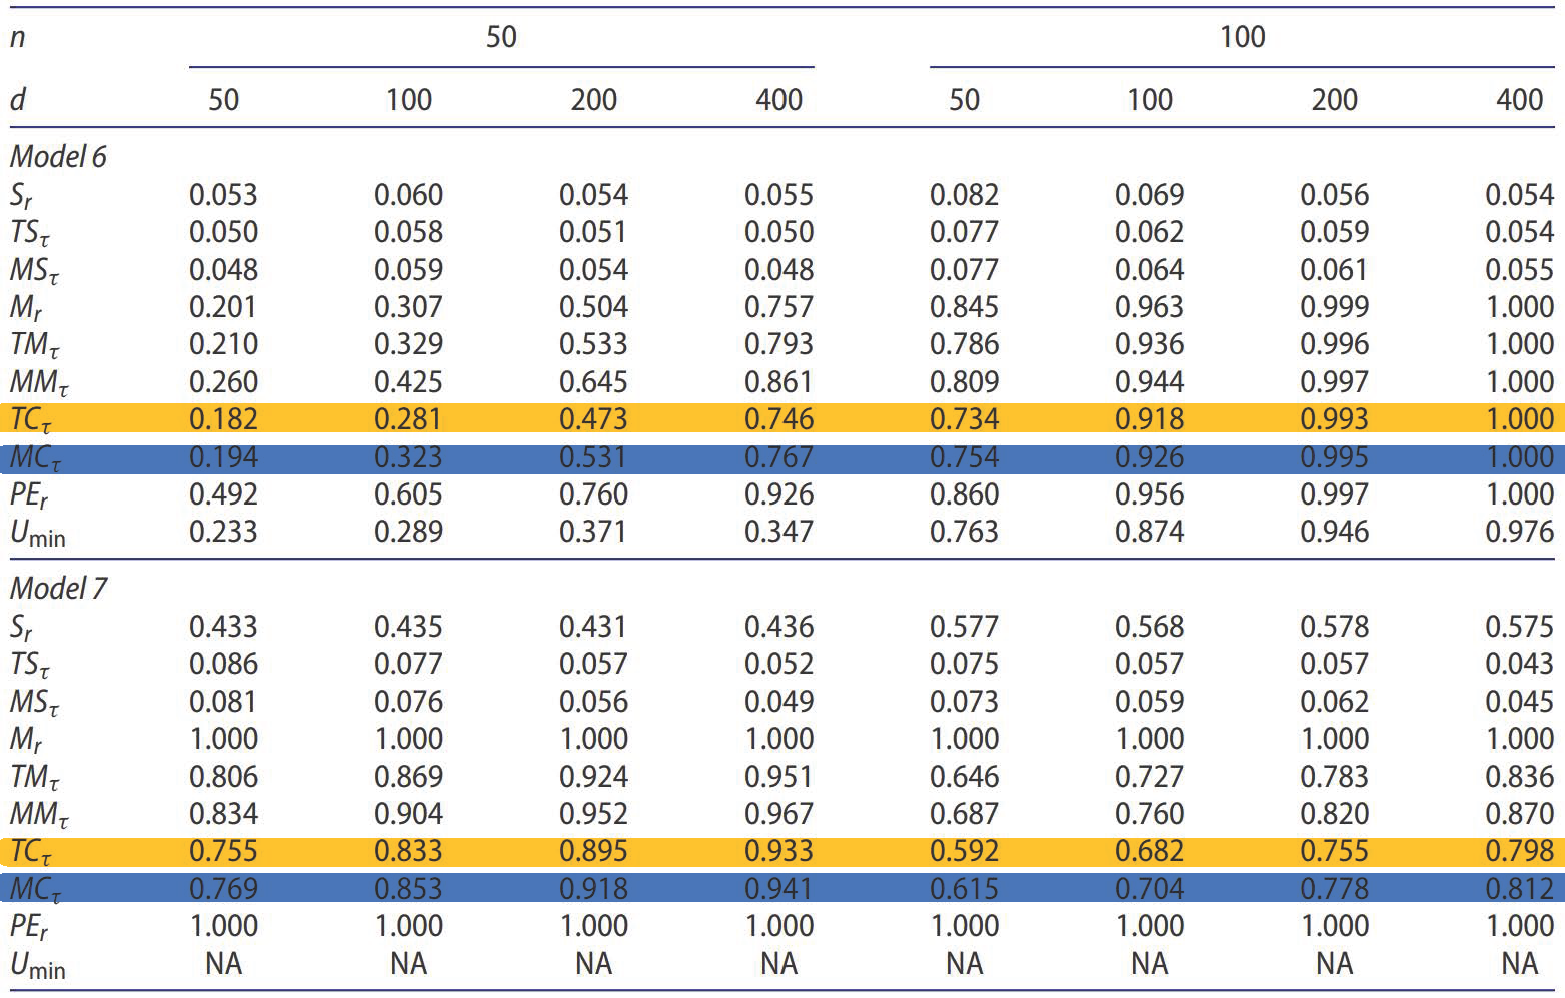
\includegraphics[width=0.8\linewidth]{Figures/Table3H} 

}

\caption{Empirical powers of tests in sparse cases.}\label{fig:Table 3}
\end{figure}
\end{frame}

\begin{frame}{Results VI}
\phantomsection\label{results-vi}
\begin{figure}

{\centering 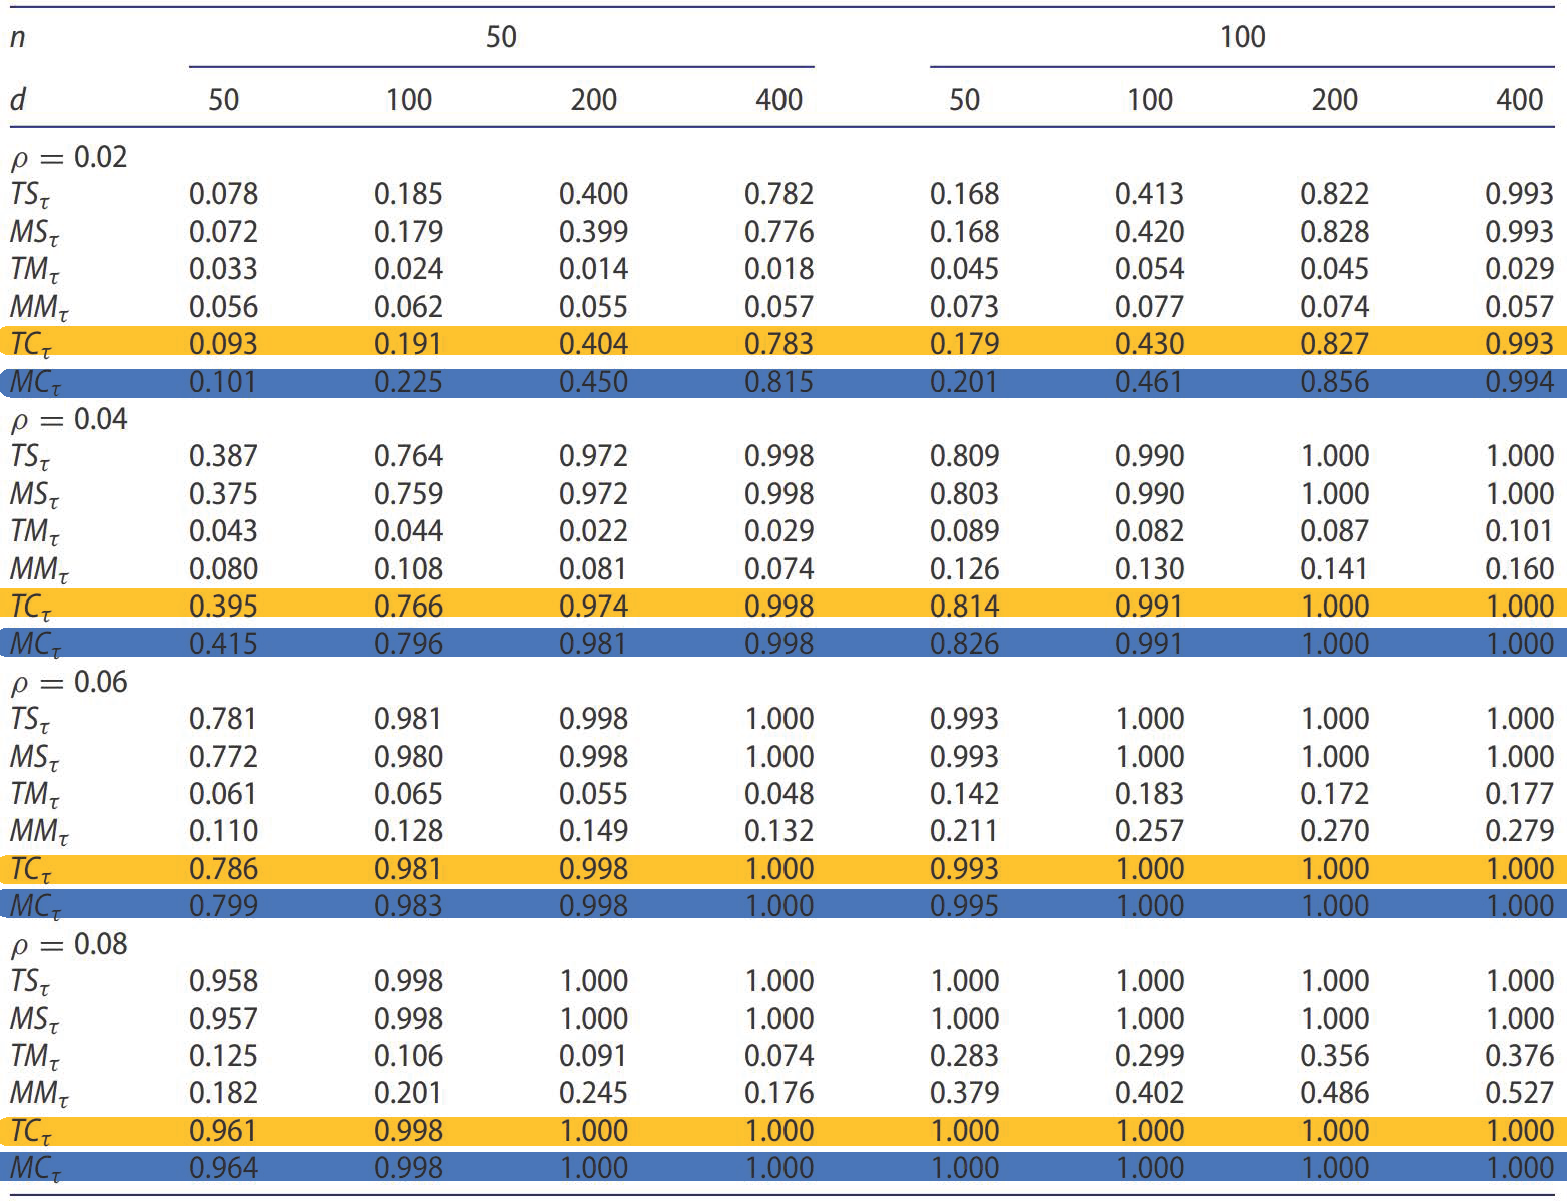
\includegraphics[width=0.8\linewidth,height=0.77\textheight]{Figures/Table4H} 

}

\caption{Empirical powers under various strengths of dependence in dense cases.}\label{fig:Table 4}
\end{figure}
\end{frame}

\begin{frame}{Results VII}
\phantomsection\label{results-vii}
\begin{figure}

{\centering 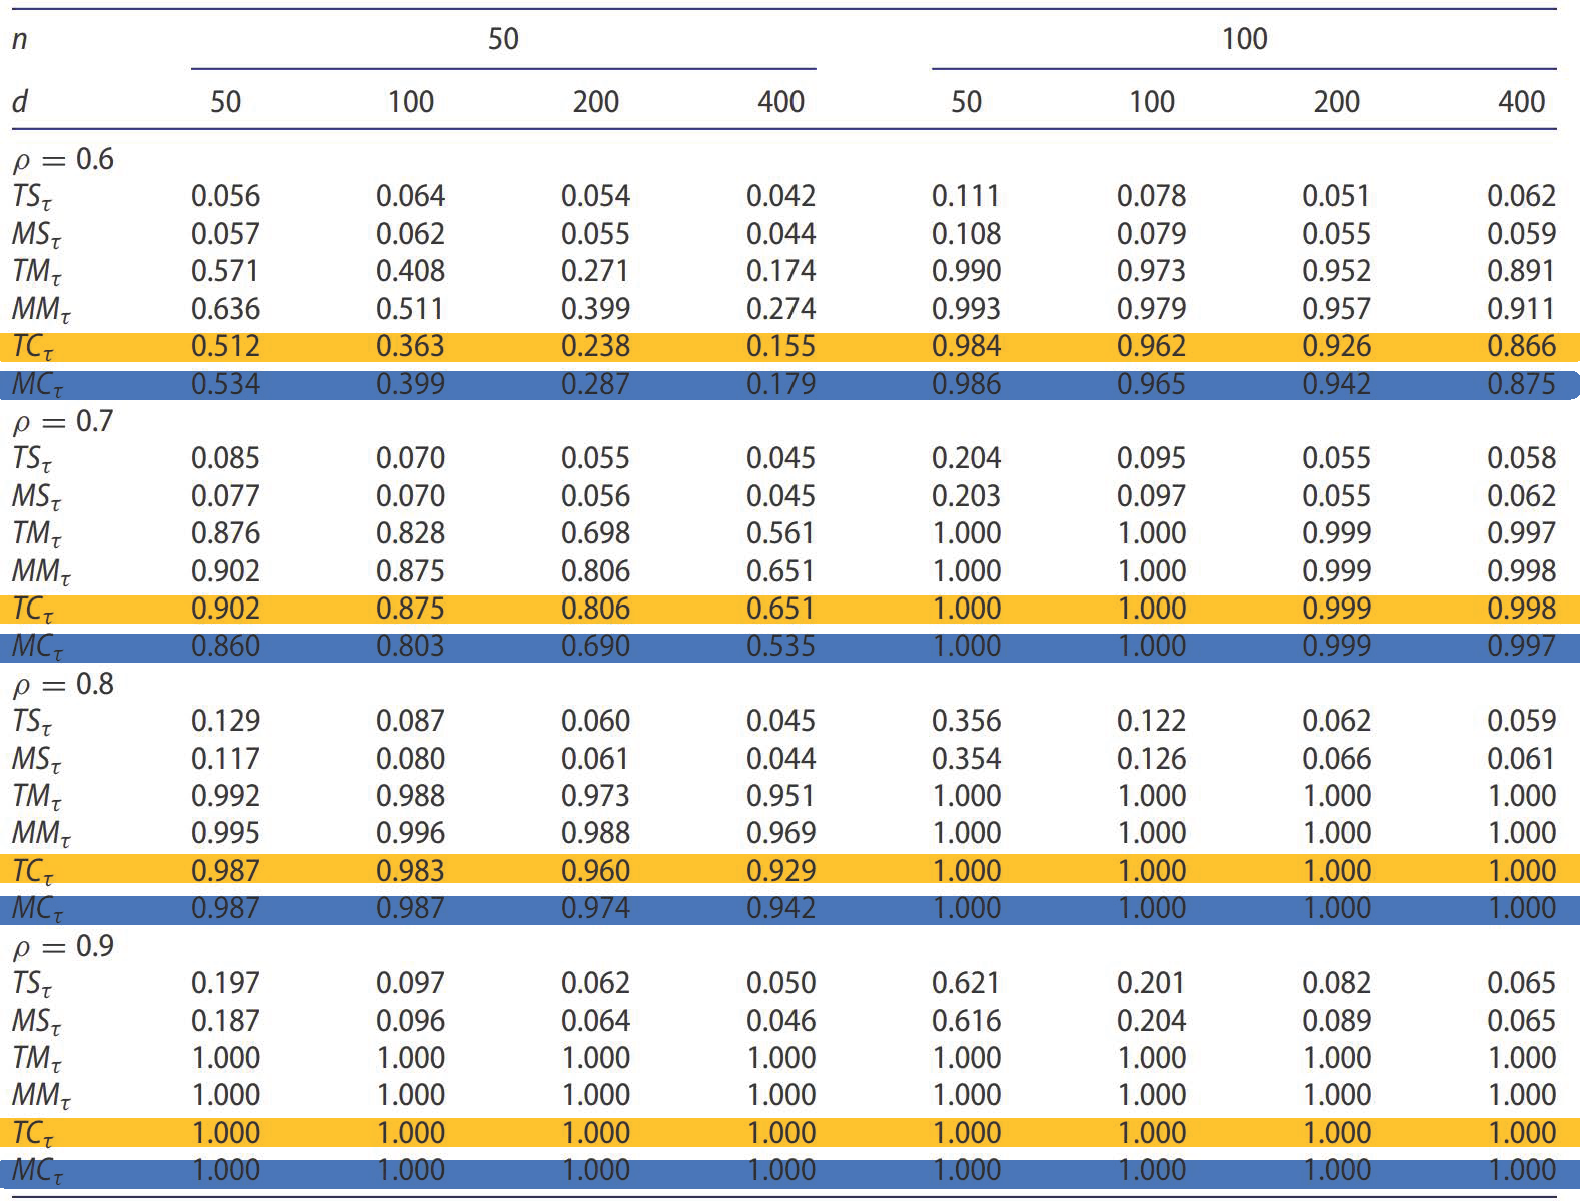
\includegraphics[width=0.8\linewidth]{Figures/Table5H} 

}

\caption{Empirical powers under various strengths of dependence in sparse cases.}\label{fig:Table 5}
\end{figure}
\end{frame}

\begin{frame}{Applications}
\phantomsection\label{applications}
\begin{itemize}
\tightlist
\item
  The paper also applies the method to two ``real-world'' examples:

  \begin{itemize}
  \tightlist
  \item
    \textbf{Welding (4 vars, n=40):} rank-based rejects null hypothesis;
    Pearson fails to reject.
  \item
    \textbf{Biochemical (8 vars, n=12):} adaptive detects group
    differences.
  \end{itemize}
\item
  I also implemented the method myself (and validated against the
  author's own method)

  \begin{itemize}
  \tightlist
  \item
    Applied (mainly for fun) to a Consulting Case
  \item
    Apriori believed the covariate to be independent, and they were (at
    least according to the adaptive test)!
  \end{itemize}
\end{itemize}
\end{frame}

\begin{frame}{Conclusion}
\phantomsection\label{conclusion}
\begin{itemize}
\tightlist
\item
  Kendall's \(\tau\) connects classic nonparametric tests to modern
  high-dimension inference.
\item
  Rank-based adaptive tests are practical and robust; 2025 work
  generalizes to sum-of-powers (Han, Ma, and Xie 2025).
\item
  We should consider this test when we know we have high-dimensional
  data, but don't know whether it is dense or sparse.
\item
  Allows us to test for independence beyond the typical ``data
  collection assessment'' and ``variable relations graphs''
\end{itemize}
\end{frame}

\begin{frame}[allowframebreaks]{References}
\phantomsection\label{references}
\scriptsize

\phantomsection\label{refs}
\begin{CSLReferences}{1}{0}
\bibitem[\citeproctext]{ref-ElShaarawi1992}
El-Shaarawi, A. H., and Stefan P. Niculescu. 1992. {``On Kendall's Tau
as a Test of Trend in Time Series Data.''} \emph{Environmetrics} 3 (4):
385--411.

\bibitem[\citeproctext]{ref-Fechner1897}
Fechner, Gustav Theodor. 1897. \emph{Kollektivmasslehre}. Leipzig:
Verlag von Wilhelm Engelmann.
\url{https://www.google.com/books/edition/Kollektivmasslehre/bgQZAAAAMAAJ?hl=en}.

\bibitem[\citeproctext]{ref-Hamed2011}
Hamed, K. H. 2011. {``The Distribution of Kendall's Tau for Testing the
Significance of Cross-Correlation in Persistent Data.''}
\emph{Hydrological Sciences Journal} 56 (5): 841--53.
\url{https://doi.org/10.1080/02626667.2011.586948}.

\bibitem[\citeproctext]{ref-Han2025}
Han, Lijuan, Yun Ma, and Junshan Xie. 2025. {``An Adaptive Test of the
Independence of High-Dimensional Data Based on Kendall Rank Correlation
Coefficient.''} \emph{Journal of Nonparametric Statistics} 37 (3):
632--56. \url{https://doi.org/10.1080/10485252.2024.2435852}.

\bibitem[\citeproctext]{ref-Kendall1938}
Kendall, M. G. 1938. {``A New Measure of Rank Correlation.''}
\emph{Biometrika} 30 (1/2): 81--93.
\url{https://www.jstor.org/stable/2332226}.

\bibitem[\citeproctext]{ref-Kruskal1958}
Kruskal, William H. 1958. {``Ordinal Measures of Association.''}
\emph{Journal of the American Statistical Association} 53 (284):
814--61. \url{https://doi.org/10.1080/01621459.1958.10501481}.

\bibitem[\citeproctext]{ref-Shi2024}
Shi, Xiangyu, Yuanyuan Jiang, Jiang Du, and Zhuqing Miao. 2024. {``An
Adaptive Test Based on Kendall's Tau for Independence in High
Dimensions.''} \emph{Journal of Nonparametric Statistics} 36 (4):
1064--87. \url{https://doi.org/10.1080/10485252.2023.2296521}.

\end{CSLReferences}
\end{frame}

\end{document}
